%%%%%%%%%%%%%%%%%%%%%%%%%%%%%%%%%%%%%%%%
\begin{figure}[thb]
\centering
% 
\begin{subfigure}[b]{0.45\linewidth}
\centering
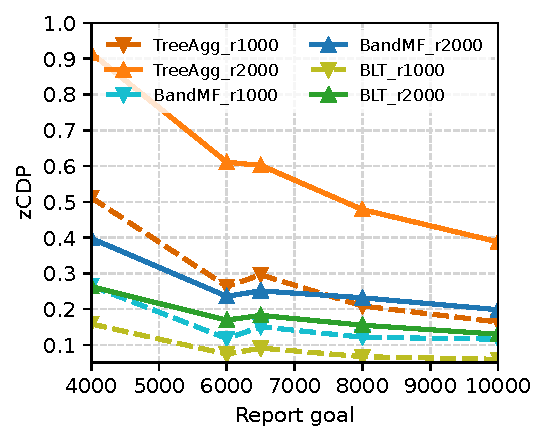
\includegraphics[width=\textwidth]{images/blt_pop3m.pdf}
\caption{\small Population 3M}
\label{fig:pop3m}
\end{subfigure}
%
\begin{subfigure}[b]{0.45\linewidth}
\centering
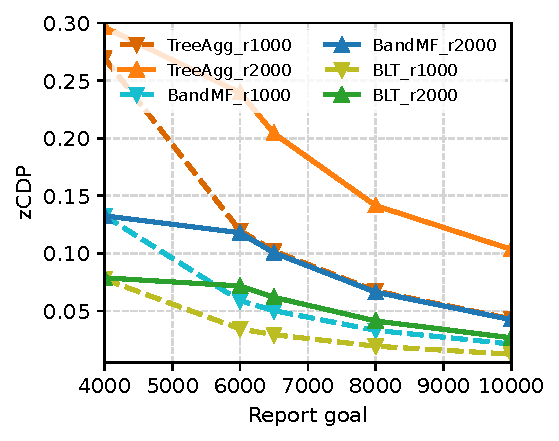
\includegraphics[width=\textwidth]{images/blt_pop10m.pdf}
\caption{\small Population 10M}
\label{fig:pop10m}
\end{subfigure}
%
\begin{subfigure}[b]{0.45\linewidth}
\centering
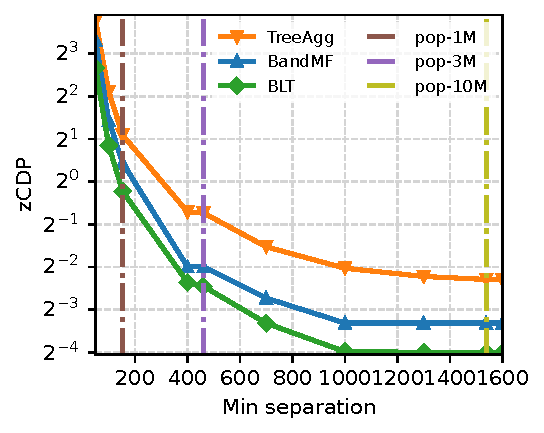
\includegraphics[width=\textwidth]{images/blt_min_sep.pdf}
\caption{\small Report goal 6500, worst-case max-par}
\label{fig:min_sep}
\end{subfigure}
%
\begin{subfigure}[b]{0.45\linewidth}
\centering
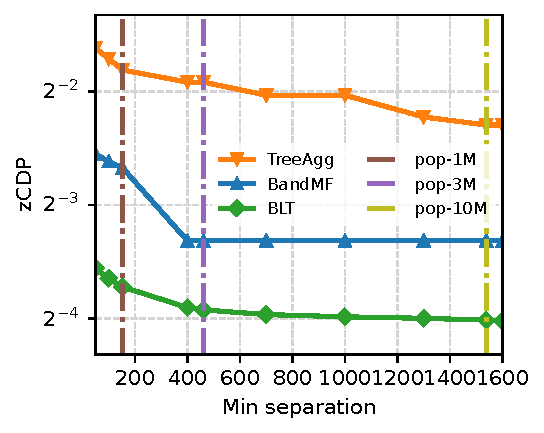
\includegraphics[width=\textwidth]{images/min_sep_max2.pdf}
\caption{\small Report goal 6500, optimistic max-par=2}
\label{fig:min_sep_max2}
\end{subfigure}
%
\caption{\small The effect of population size, number of rounds, report goals, and min-seps on DP-FTRL privacy guarantees. The results are extrapolate from the setting for es-ES and id-ID (\bandmf and \blt matrices are optimized for min-sep=400) based on the hypothesis that linearly scale noise multiplier and report goal, or only change min-sep will not affect the model utility. The For a fixed number of rounds to achieve utility target, increasing report goal and min-sep can achieve stronger guarantees measured by smaller zCDP. The optimal min-sep is capped by population size for a fixed report goal, and \blt provides better guarantees, and smoother transition across different min-seps. 
}\label{fig:extrapolate}
\end{figure}
%%%%%%%%%%%%%%%%%%%%%%%%%%%%%%%%%%%%%%%%